%%%%%%%%%%%%%%%%%%%%%%%%%%%%%%%%%%%%%%%
\newcommand{\comparehelen}[2]
{
\includegraphics[width=2.5cm,height=2.5cm]{images/helen/helen_#1}                  & \hspace{0.5cm}
\includegraphics[width=2.3cm,height=2.5cm]{images/helen/helen_#1_frontal_low_rank} & \hspace{0.5cm}
\includegraphics[width=2.3cm,height=2.5cm]{images/helen/helen_#1_frontal_ira}      & \hspace{0.5cm}
\includegraphics[width=3cm,height=2.5cm]{images/helen/helen_#1_#2_low_rank}        & \hspace{0.5cm}
\includegraphics[width=3cm,height=2.5cm]{images/helen/helen_#1_#2_ira}
}
%%%%%%%%%%%%%%%%%%%%%%%%%%%%%%%%%%%%%%%
%%%%%%%%%%%%%%%%%%%%%%%%%%%%%%%%%%%%%%%
% \setlength{\tabcolsep}{1pt}
% \begin{figure*}[th]
%     \centering
%     \begin{tabular}{ccccc} \vspace*{0.2cm}
%         Input & \hspace{0.5cm} Proposed & \hspace{0.5cm}~\cite{RefWorks:311} & \hspace{0.5cm} Proposed & \hspace{0.5cm}~\cite{RefWorks:311} \\
%         \comparehelen{1348}{side}                                                                                                           \\
%         \comparehelen{555}{side}                                                                                                            \\
%         \comparehelen{680}{chin}                                          
%     \end{tabular}
%     \caption{{\bf Comparison with the blind decomposition of~\cite{RefWorks:311}}.
%              Images from the HELEN~\cite{RefWorks:318} dataset.}
% \label{fig:helen_compare}
% \end{figure*}
% \setlength{\tabcolsep}{6pt}
%%%%%%%%%%%%%%%%%%%%%%%%%%%%%%%%%%%%%%%
%%%%%%%%%%%%%%%%%%%%%%%%%%%%%%%%%%%%%%%
\begin{table}[th]
    \centering
    \begin{tabular}{lccccc}
        \toprule
        Data   & W1 & Train & W2 & Tot \\ \midrule
        HELEN (2330)    & 8       & 730       & 25        & 763   \\
        T. Hanks (274)  & 1       & 21        & 4         & 26    \\  \bottomrule
    \end{tabular}
    \caption{\textbf{Training Times.} Mean training times in seconds over 10
             runs rounded to the nearest second. ``W1'' denotes warping to the
             LFPW reference frame of $(150 \times 150)$ pixels, ``W2'' denotes
             warping back to the original images and ``Train'' denotes the total
             training time of our method described in
             \cref{subsec:robust_sh_basis}. Original images were larger than 
             the reference, hence the increase from ``W1'' to ``W2''. Timings
             were recorded on an Intel Xeon E5--1650 3.20GHz with 32GB of RAM.}
\label{tbl:timings}
\end{table}
%%%%%%%%%%%%%%%%%%%%%%%%%%%%%%%%%%%%%%%
%%%%%%%%%%%%%%%%%%%%%%%%%%%%%%%%%%%%%%%%%%%%%%%%%%%%%%%%%%%%%%%%%%%%%%%%%%%%%%%%
\section{Experiments}\label{sec:imag_coll_experiments}
%%%%%%%%%%%%%%%%%%%%%%%%%%%%%%%%%%%%%%%%%%%%%%%%%%%%%%%%%%%%%%%%%%%%%%%%%%%%%%%%
In this section we provide a number of experiments that emphasise the increased
robustness of our reconstructions. We also show a new application to this type
of model that involves improving the fitting results of an AAM using our
constructed SH basis. Choosing the number of components, $k$, to recover is an
important problem that was not properly addressed by Kemelmacher-Schlizerman in
\cite{RefWorks:311}. In these experiments we attempt to recover as many
components as possible in order to strike a balance between cleanly
reconstructed normals and identity. However, there is a trade-off when choosing
the value of $k$. In particular, if the value of $k$ is too large, then the
decomposition is unable to separate the identity and shape and the subspace of
shape no longer represents valid normals. This is one of the primary advantages
of our robust decomposition, as it allows the value of $k$ to be larger given
the reduced rank of the images. However, a potential disadvantage of our
proposed method is the sensitivity of the algorithm to the parameter $\lambda$,
which must be tuned for every dataset. It is also important to stress that our
main goal is to recover the low frequency shape information to provide plausible
3D facial surfaces under challenging conditions. However, in
\cref{subsec:experiments_smith}, we show that our recovered subspace can
be used in existing high frequency recovery algorithms such as SFS.\@

The area of 3D facial surface recovery is lacking any form of formal
quantitative benchmark. The quantitative benchmark presented in
\cite{RefWorks:311} is performed on depth data recovered from photometric
stereo. This is not ground truth depth data, as error is introduced during
integration, and a more accurate evaluation would be the angular error of the
recovered normals. However, in the presence of cast shadows, even the normals of
photometric stereo are biased. For this reason, the lack of a standard and fair
quantitative evaluation, we focus on qualitative results in this paper.

Specifically we performed the following experiments: (1) We built our subspace
using the HELEN~\cite{RefWorks:318} dataset. We directly compare against the
blind decomposition proposed in~\cite{RefWorks:311} and show particularly
challenging images from the dataset. This experiment highlights the difficulty
in constructing subspaces from large a set of in-the-wild images. (2) We show
that the robust subspace learnt in (1) can be used within the shape-from-shading
(SFS) framework of \citet{RefWorks:90}. By recovering the normals
from every image of HELEN, we can perform a secondary principal component
analysis (PCA) on the normals in order to directly embed them within Smith's
algorithm. In this experiment, we compare against a clean dataset of normals
acquired from the ICT-3DRFE~\cite{Stratou:2012jh} database. (3) We show how our
subspace can be combined with an existing facial alignment algorithm, namely
project-out AAMs~\cite{RefWorks:227}. Our subspace can be used both as the
appearance basis for the AAM and also as a methodology of recovering dense 3D
shape.

In the following section we describe the construction of the bases and explain
what processing was performed on each dataset.
%%%%%%%%%%%%%%%%%%%%%%%%%%%%%%%%%%%%%%%%%%%%%%%%%%%%%%%%%%%%%%%%%%%%%%%%%%%%%%%%
\subsection{Constructing The Robust Bases}\label{subsec:construction}
%%%%%%%%%%%%%%%%%%%%%%%%%%%%%%%%%%%%%%%%%%%%%%%%%%%%%%%%%%%%%%%%%%%%%%%%%%%%%%%%
The process of building the robust SH basis was the same for all datasets
involved. Facial annotations consisting of 68 points were recovered through
various methods for each dataset. In the case of the HELEN database, the manual
annotations provided by the IBUG group were used~\cite{Sagonas:et,Sagonas:fn},
in the case of the Yale B, Photoface and ICT-3DRFE databases, manual annotations
were used and the in-the-wild images and video of Tom Hanks were automatically
annotated by the one millisecond facial alignment method of~\cite{Kazemi:he}
provided by the Dlib project~\cite{dlib09}.

These annotations were then warped via a Piecewise Affine transformation to a
mean reference shape that was built from all the faces, training and testing, of
the LFPW facial annotations provided by IBUG.\@ This provided the dense
correspondence required for performing matrix decompositions. To construct our
SH bases, we performed the algorithm as described in
\cref{subsec:robust_sh_basis} on the warped images. In order to provide
the example reconstructions, the reconstructed images were warped back into
their original shapes and then integrated using the method of 
\citet{RefWorks:99}.

\cref{tbl:timings} gives examples of the training time taken for the in-
the-wild Tom Hanks images and the HELEN dataset. It is important to note that
part of the reason the training time is much lower for the Tom Hanks images is
that they have an inherently lower rank than the HELEN images as they are all of
the same individual. This greatly affects the convergence time and thus the
timings do not scale linearly.
%%%%%%%%%%%%%%%%%%%%%%%%%%%%%%%%%%%%%%%%%%%%%%%%%%%%%%%%%%%%%%%%
\subsection{Comparison Using HELEN}\label{subsec:experiments_helen}
%%%%%%%%%%%%%%%%%%%%%%%%%%%%%%%%%%%%%%%%%%%%%%%%%%%%%%%%%%%%%%%%
In this set of experiments we wished to convey two results: (1) that we are
capable of quickly constructing our basis on a large number of in-the-wild
images, (2) that the our robust formulation of the problem gives superior
performance to the blind decomposition used by~\cite{RefWorks:311}. In this
experiment, $k = 200$ and the total number of components was thus $4k = 800$.
\cref{fig:helen_compare} shows the results from this experiment. As we can
clearly see, on challenging images the blind decomposition is unable to separate
the appearance from the illumination and thus the recovered normals are unable
to recover accurate shape.
%%%%%%%%%%%%%%%%%%%%%%%%%%%%%%%%%%%%%%%%%%%%%%%%%%%%%%%%%%%%%%%%
\subsection{Using The Subspace In SFS}\label{subsec:experiments_smith}
%%%%%%%%%%%%%%%%%%%%%%%%%%%%%%%%%%%%%%%%%%%%%%%%%%%%%%%%%%%%%%%%
The SFS technique of \citet{RefWorks:90} relies on a PCA basis
constructed from normals of a single class of object. It then seeks to recover
the high frequency normal information directly from the texture. In order to
create the PCA required by~\cite{RefWorks:90}, we recovered spherical harmonics
for every image in the dataset using the proposed algorithm. We then computed
Kernel-PCA~\cite{Snape:2014de} on the normals recovered from the HELEN images
and supplied them to~\cite{RefWorks:90}. The lighting vector is also an input to
the algorithm and we recover it by solving a least squares problem with the
known mean normals.

In order to provide a comparison for our reconstruction, we created a clean
normal subspace using the data from the ICT-3DRFE~\cite{Stratou:2012jh}
database. This database is primarily use for image relighting purposes, however,
they provide a very accurate set of normals of faces under a wide range of
expressions. The results of this experiment are shown in \cref{fig:smith}.
Although our subspace did not provide reconstructions that are as visually
accurate as the subspace from ICT-3DRFE, they were still able to successfully
recover a plausible representation of the high frequency shading information.
%%%%%%%%%%%%%%%%%%%%%%%%%%%%%%%%%%%%%%%%%%%%%%%%%%%%%%%%%%%%%%%%
\subsection{Automatic Alignment}\label{subsec:experiments_alignment}
%%%%%%%%%%%%%%%%%%%%%%%%%%%%%%%%%%%%%%%%%%%%%%%%%%%%%%%%%%%%%%%%
%%%%%%%%%%%%%%%%%%%%%%%%%%%%%%%%%%%%%%%
\newcommand{\tomhanksalignment}[1]
{
\includegraphics[width=2.3cm,height=2.5cm]{images/tom_hanks/tom_hanks_improve_#1_initial} &
\includegraphics[width=2.3cm,height=2.5cm]{images/tom_hanks/tom_hanks_improve_#1_final}   & \hspace{0.3cm}
\includegraphics[width=2cm,height=2.5cm]{images/tom_hanks/tom_hanks_improve_#1_depth}
}
%%%%%%%%%%%%%%%%%%%%%%%%%%%%%%%%%%%%%%%
%%%%%%%%%%%%%%%%%%%%%%%%%%%%%%%%%%%%%%%
% \setlength{\tabcolsep}{1pt}
% \begin{figure}[t]
%     \centering
%     \begin{tabular}{ccc}
%         Initial & Final & \hspace{0.3cm} Recovered Depth \\
%         \tomhanksalignment{1}             \\
%         \tomhanksalignment{129}
%     \end{tabular}
%     \caption{{\bf Person specific model fitting for Tom Hanks}. Images of Tom 
%              Hanks coarsely aligned by a facial alignment method. Our algorithm 
%              improves the facial alignment and simultaneously recovers depth. 
%              Images shown are from a YouTube video of Tom Hanks.}
% \label{fig:improve_tom_hanks}
% \end{figure}
% \setlength{\tabcolsep}{6pt}
%%%%%%%%%%%%%%%%%%%%%%%%%%%%%%%%%%%%%%%
%%%%%%%%%%%%%%%%%%%%%%%%%%%%%%%%%%%%%%%
% \begin{figure}[t]
%     \centering
%     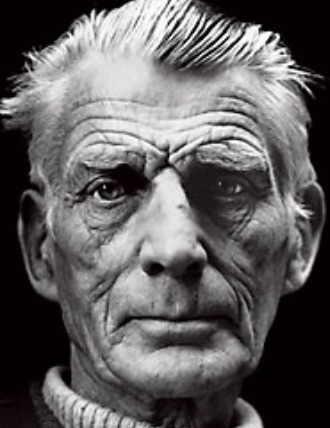
\includegraphics[width=2cm,height=2.5cm]{images/smith/samuel_beckett}                    \hspace{0.3cm}
%     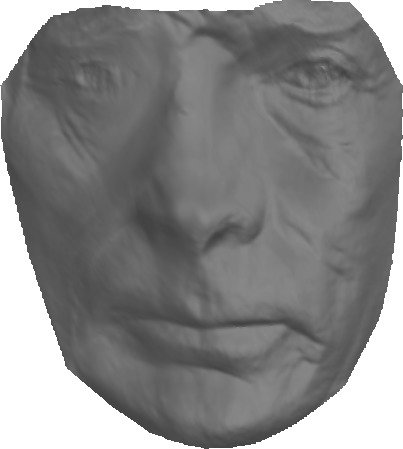
\includegraphics[width=2cm,height=2.5cm]{images/smith/beckett_smith_frontal_ict}         \hspace{0.3cm}
%     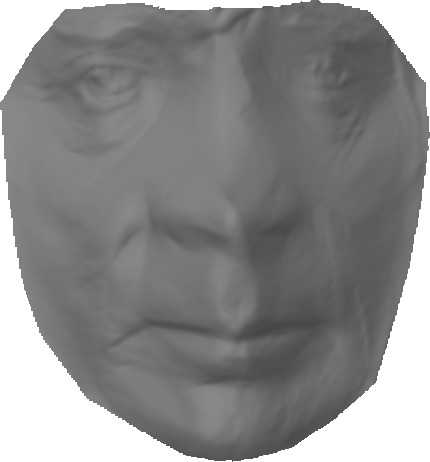
\includegraphics[width=2cm,height=2.5cm]{images/smith/beckett_smith_frontal_low_rank} \\
%     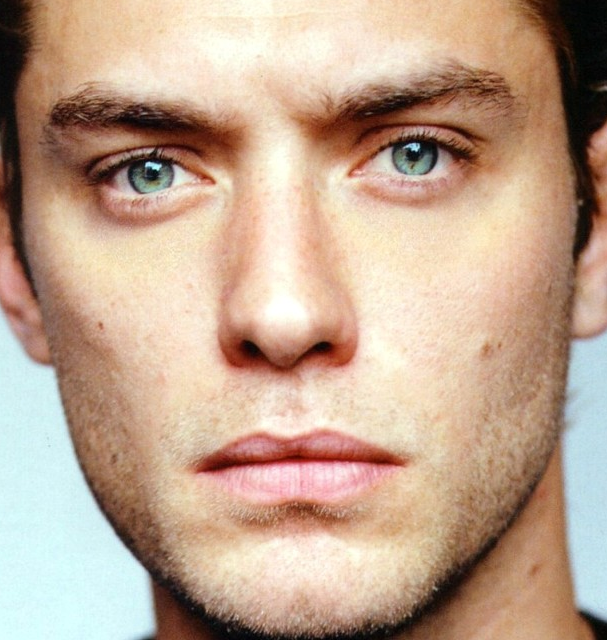
\includegraphics[width=2cm,height=2.5cm]{images/smith/jude_law}                          \hspace{0.3cm}
%     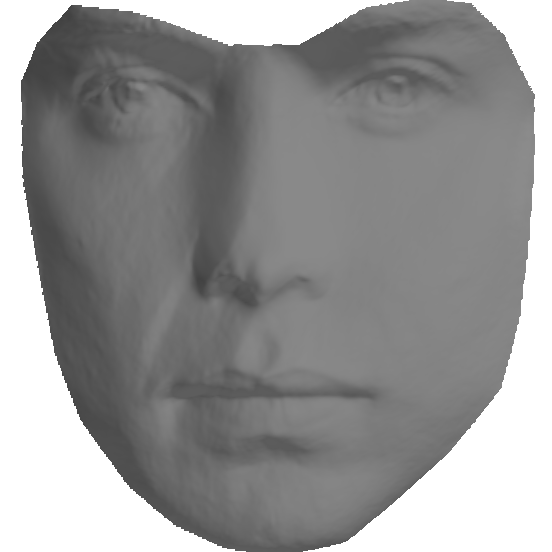
\includegraphics[width=2cm,height=2.5cm]{images/smith/law_smith_frontal_ict}             \hspace{0.3cm}
%     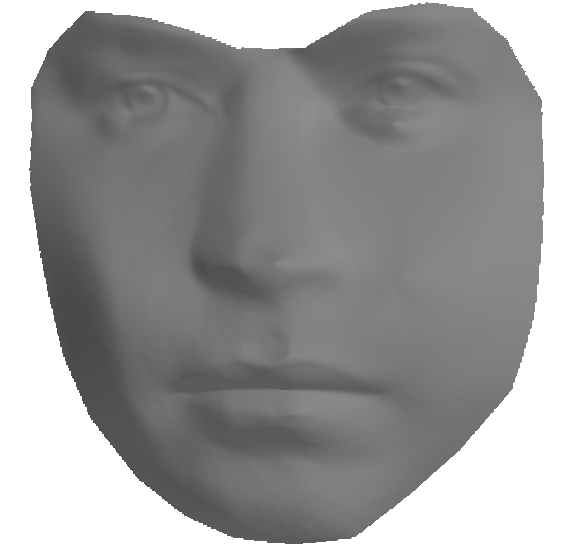
\includegraphics[width=2cm,height=2.5cm]{images/smith/law_smith_frontal_low_rank}
%     \caption{{\bf Our subspace used for SFS}. Normals learnt automatically from 
%              the SH subspace of HELEN vs normals from the clean data of 
%              ICT-3DRFE.\@ Middle column: the clean data. 
%              Right column: proposed subspace.}
% \label{fig:smith}
% \end{figure}
%%%%%%%%%%%%%%%%%%%%%%%%%%%%%%%%%%%%%%%
In this experiment we used the Active Template Model (ATM) provided by the Menpo
project~\cite{menpo14} in order to perform a project-out type algorithm to align
images of Tom Hanks. This model is similar to the Lucas-Kanade
\cite{RefWorks:71} method but uses a point distribution model (PDM) in order to
perform non-rigid alignment between the images. In particular, the template
image is fixed during optimisation of the PDM, and we use our subspace to
provide a texture representing an approximation of the diffuse component of the
image. This is essentially identical to the procedure performed within a
project-out AAM.\@

We used a person specific SH subspace that was built on images of Tom Hanks that
were downloaded automatically from the Internet. In this case, the images were
automatically aligned using the DLib implementation of~\cite{Kazemi:he}. For
this experiment, $k = 30$ and thus the total number of components $4k = 120$. We
downloaded 200 frames from a Youtube video of Tom
Hanks\footnote{\url{https://www.youtube.com/watch?v=nFvASiMTDz0} from 3:43} and
attempted to automatically align them using our subspace and the ATM.\@ The ATM
was initialised using another fitting of~\cite{Kazemi:he} which was then
iteratively improved. At each global iteration, we recovered a new set of
diffuse textures for each frame and then performed a refitting of every frame.
This caused the images to align over a sequence of iterations. We performed 10
such iterations. \cref{fig:improve_tom_hanks} shows two example frames
where the alignment was improved and dense shape was also recovered.